\documentclass[journal]{IEEEtran}


\usepackage[pdftex]{graphicx}
\usepackage{amsmath}
\usepackage{algorithm}
\usepackage[noend]{algpseudocode}
\usepackage{array}
\usepackage{subcaption}
% correct bad hyphenation here
\hyphenation{op-tical net-works semi-conduc-tor}


\begin{document}
%
% paper title
% Titles are generally capitalized except for words such as a, an, and, as,
% at, but, by, for, in, nor, of, on, or, the, to and up, which are usually
% not capitalized unless they are the first or last word of the title.
% Linebreaks \\ can be used within to get better formatting as desired.
% Do not put math or special symbols in the title.
\title{Detection and Instance Segmentation of Neuroblastoma Cells using YOLO, UNet and Conditional Random Fields}

\author{Kristofer delas Pe\~nas and
        Dominic Waithe% <-this % stops a space
\thanks{K. delas Pe\~nas is with the Doctoral Training Centre, University of Oxford, United Kingdom, and the Department of Computer Science, University of the Philippines Diliman, Philippines e-mail: \texttt{kristofer.delaspenas@wolfson.ox.ac.uk}.}% <-this % stops a space
\thanks{D. Waithe is with the MRC Weatherall Institute of Molecular Medicine, University of Oxford, United Kingdom.}}% <-this % stops a space

% The paper headers
\markboth{Oxford-Nottingham Centre for Doctoral Training for Biomedical Imaging}%
{delas Pe\~nas: Detection and Semantic Segmentation of Neuroblastoma Cells using YOLO, UNet and Conditional Random Fields}
% The only time the second header will appear is for the odd numbered pages
% after the title page when using the twoside option.
% 
% *** Note that you probably will NOT want to include the author's ***
% *** name in the headers of peer review papers.                   ***
% You can use \ifCLASSOPTIONpeerreview for conditional compilation here if
% you desire.




% If you want to put a publisher's ID mark on the page you can do it like
% this:
%\IEEEpubid{0000--0000/00\$00.00~\copyright~2015 IEEE}
% Remember, if you use this you must call \IEEEpubidadjcol in the second
% column for its text to clear the IEEEpubid mark.



% use for special paper notices
%\IEEEspecialpapernotice{(Invited Paper)}




% make the title area
\maketitle

% As a general rule, do not put math, special symbols or citations
% in the abstract or keywords.
\begin{abstract}
The abstract goes here.
\end{abstract}

% Note that keywords are not normally used for peerreview papers.
\begin{IEEEkeywords}
IEEE, IEEEtran, journal, \LaTeX, paper, template.
\end{IEEEkeywords}






% For peer review papers, you can put extra information on the cover
% page as needed:
% \ifCLASSOPTIONpeerreview
% \begin{center} \bfseries EDICS Category: 3-BBND \end{center}
% \fi
%
% For peerreview papers, this IEEEtran command inserts a page break and
% creates the second title. It will be ignored for other modes.
\IEEEpeerreviewmaketitle



\section{Introduction}
\IEEEPARstart{T}{his} demo file is intended to serve as a ``starter file''
for IEEE journal papers produced under \LaTeX\ using
IEEEtran.cls version 1.8b and later.
% You must have at least 2 lines in the paragraph with the drop letter
% (should never be an issue)
I wish you the best of success.

\section{Literature Review}
\subsection{Semantic Segmentation}
Semantic segmentation describes the process of assigning each pixel of an image a class label, such as dog, sky, or car. It is one of the key problems in computer vision. Through semantic segmentation, applications requiring scene understanding can be built, like self-driving vehicles and virtual reality. 

In recent years, as a natural progression of the popularity of applications of convolutional neural networks (CNN), several CNN-based architectures were developed for semantic segmentation. A step further from the classification problems addressed by CNN architectures like AlexNet, VGG, Inception and ResNet, architectures coupling classification with localization, detection, and segmentation were built. Most of these segmentation architectures were designed as \textit{encoder-decoder} models. The \textit{encoder} is a classification network, oftentimes utilising the aforementioned popular CNN architectures. This network \textit{learns} discriminative features for segmentation in a lower-dimensional space. To achieve a full-resolution segmentation, the output of the \textit{encoder} is passed to the \textit{decoder} that would project it back to the original resolution space.
\subsection{Instance Segmentation}
Instance segmentation builds on top of semantic segmentation. Not only are class labels assigned to each pixel, instances of the same class were also discriminated. This addresses problems beyond simple scene understanding, where quantification and individuality of objects is needed. One key issue that algorithms for instance segmentation are still trying to improve on is the resolution of overlapping instances.
\subsection{YOLO}
The YOLO (You Only Look Once) network \cite{redmon2016yolo9000} is a state-of-the-art object detection system that gained popularity within the past few years. It employs a series of convolutions to detect and localize objects in real-time.

The implementation of YOLO starts with an initial 416 $\times$ 416 image input. The system performs 19 convolutions with an overall downsampling factor of 32, resulting to an output feature map of 13 $\times$ 13 dimension which is used to predict the bounding boxes of detected objects with the help of anchor boxes.

With version 2 of YOLO, \cite{redmon2016yolo9000} demonstrated a high mean average precision (mAP) on the VOC dataset, higher than existing architectures like Faster-RCNN.

A more recent YOLO iteration, version 3 \cite{yolov3}, uses a deeper network and performs object detection on 3 stages of different resolutions. With these changes, an even higher mAP was achieved, however, at the expense of heavier computational resource requirement and longer detection time.
\subsection{UNet}
UNet\cite{RFB15a} is a fully convolutional neural network architecture that aims to semantically label individual pixels in the image. The network consists of two paths - a contracting path and an expansive path. The contracting path is the typical convolutional network with a series of convolutional layers with rectified linear unit (ReLU) activations and pooling layers to downsample.

The expansive path is an upsampling route, taking the output of the contracting path. This path performs a series of \textit{up-convolutions}, a combination of upsampling and a 2 $\times$ 2 convolution.

The key feature in UNet is the shortcut connections between the two paths for each resolution scale as shown in Figure \ref{fig:unet}. At each scale, concatenating the output from the contracting path with the upsampled output from the previous scale in the expansive path, ensures that the finer details lost through downsampling can be recovered and be used to fine tune the segmentation.

UNet was first applied on microscopy images but since then have been applied to different imaging modalities like MRIs and CT scans.
\begin{figure}
\centering
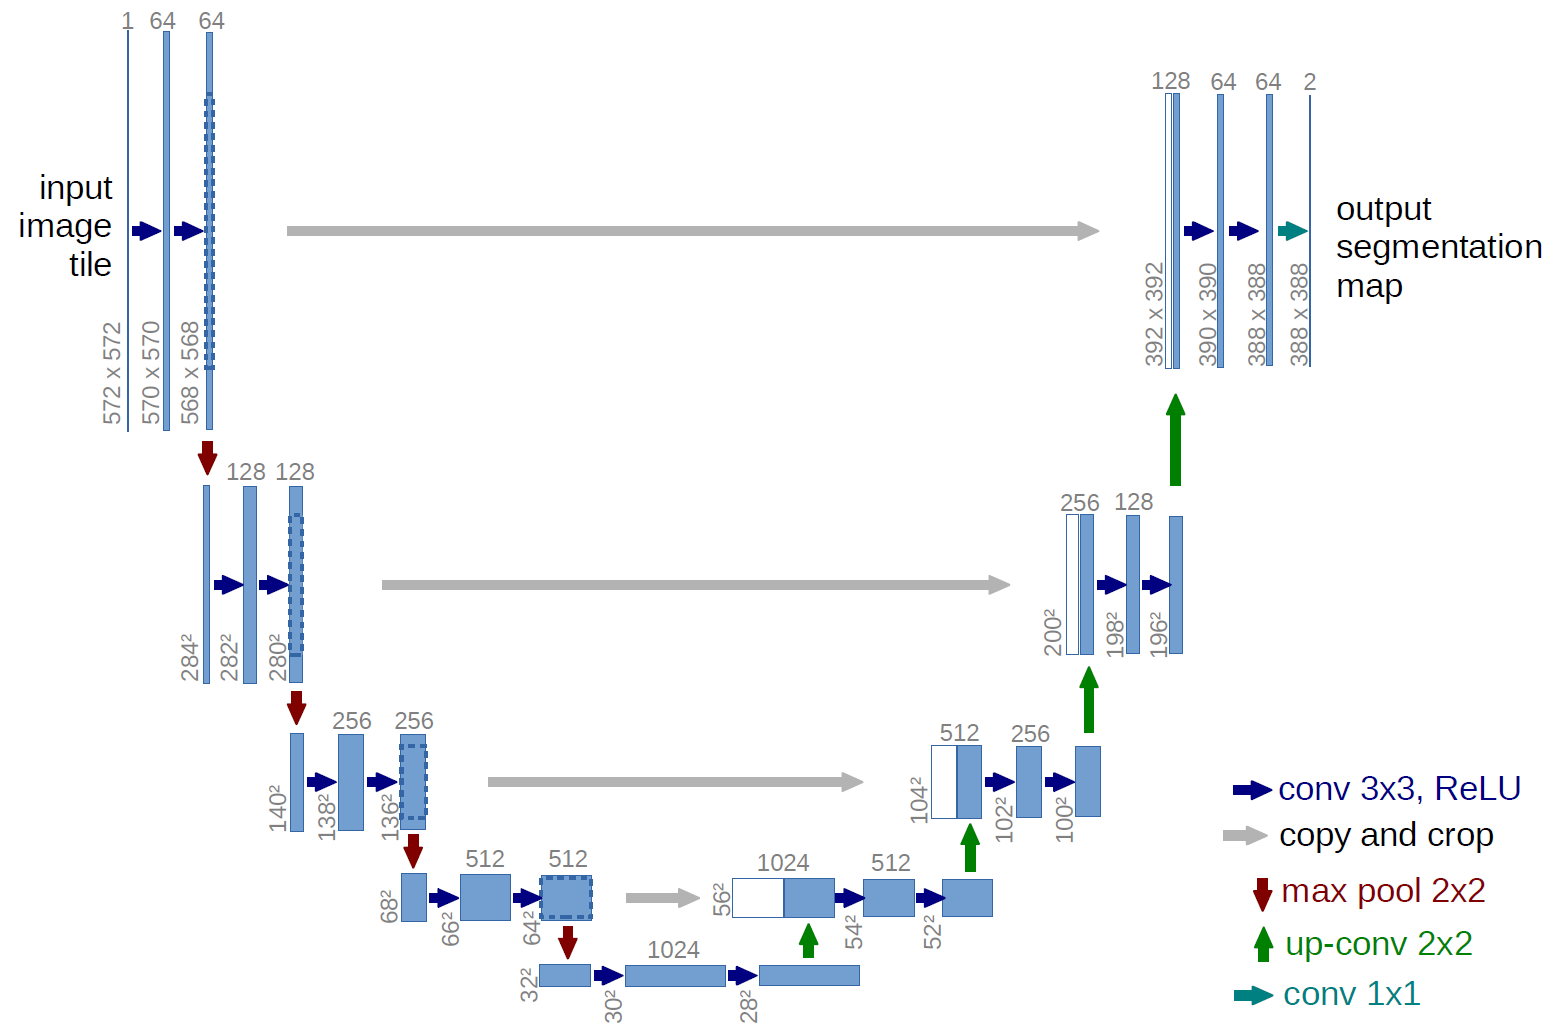
\includegraphics[width=3in]{unet.png}
\caption{\textbf{U-net architecture} \cite{RFB15a} (example for 32x32 pixels in the lowest resolution). Each blue
box corresponds to a multi-channel feature map. The number of channels is denoted
on top of the box. The x-y-size is provided at the lower left edge of the box. White
boxes represent copied feature maps. The arrows denote the different operations.}
\label{fig:unet}
\end{figure}
\subsection{Conditional Random Fields}
Many learning problems can be described as a graphical model. In artificial intelligence, one common way to model these problems is a probabilistic approach wherein probability distributions \textit{$\Psi$} are assigned over the random variables \textit{Y}. Formally, the problem can be modelled as the product of all \textit{$\Psi_i$} distributions
\begin{equation}
p(Y) = \frac{1}{Z}\prod_1^A \Psi_a(y_a)
\end{equation}
for factors \textit{F} = \{$\Psi_a$\} that have $\Psi_a \geq 0$. 
 
Markov networks and conditional random fields (CRF) are formulated similarly in this manner. The main difference is that the CRF learns the conditional probability $p(y|x)$ while Markov networks ultimately obtain the joint probability $p(y,x)$. With the joint probability $p(y,x)$, models like the Markov networks can describe the hypothesis space through the generation of all possible features \textit{x} for all labels \textit{y}. However, joint probability $p(y,x)$ involves prior knowledge on or estimate for $p(x)$, and the dependence (or independence) of the random variables. For general classification tasks, however, modelling of $p(x)$ is not needed as the concern is only on assigning labels to features, which is exactly what the conditional probability $p(y|x)$ gives.

%put figure here
Exact inference on conditional random fields is computationally expensive and usually impossible. If exact inference is possible, performing naively the sum of products of potentials (\textbf{message passing}) for all variables, can take a long time, especially for dense graphs. Current implementations of CRFs perform inference by approximation, with the speedup by employing dynamic programming. One inference algorithm is the mean field inference described in Algorithm \ref{alg:meanfieldinference}.

Each iteration of the mean field inference described in Algorithm \ref{alg:meanfieldinference} performs a message passing step, compatibility transform, and local update and normalization. Each step, except the message passing, runs in linear time. Message passing is the computational bottleneck. For a naive solution, it requires summing up over all variables and runs in quadratic time. For this very reason, the conditional random fields gained the reputation of being nooriously slow and impractical for a lot of machine learning tasks, especially those involving dense graph representations like image segmentation.

%message passing as convolution
Addressing the slow inference in CRFs, \cite{NIPS2011_4296} showed that message passing can be approximated and expressed as a convolution with a Gaussian kernel as follows:
\begin{equation}
\widetilde{Q}_i^{(m)}(l)\gets \sum_{j\neq i}k^{(m)}(f_i,f_j)Q_j(l) = [G_(m) \otimes Q(l)](f_i) - Q_i(l)
\end{equation}
This approximation can be extended to higher dimensions, and with the permutohedral lattice data structure, efficient message passing can be done in $O(Nd)$ time where \textit{N} is the number of variables and \textit{d} the number of dimensions. 
%cnnasrnn
Furthermore, \cite{crfasrnn_ICCV2015} and \cite{higherordercrf_ECCV2016} demonstrated how the mean field inference in CRFs can be written as recurrent neural network with learnable weights. This formulation allows the CRFs to be seamlessly integrated as part of a convolutional neural network model for tasks such as image segmentation.

With CRFs implemented as RNNs, several research has been done applying CNN-CRFs for general image segmentation task. \cite{NIPS2011_4296} and \cite{Teichmann2018ConvolutionalCF} proposed systems using CRFs integrated in CNNs for semantic image segmentation. Both systems train the CRF by minimizing the Gibbs energy and in doing so, finding the Maximum A Posteriori labelling of the image pixels. The CRF for semantic image segmentation is formulated with the following energy function for assignment of the pixels to semantic classes,
\begin{equation}
E(X = x) = \sum_i U(x_i) + \sum_{i<j}P(x_i,x_j)
\end{equation}
where \textit{U} is the unary potential and \textit{P} the pairwise potential. In \cite{NIPS2011_4296}, responses from the TextonBoost filter bank, color, histogram of oriented gradients (HOG) and pixel location features were used for the unary potential. On the other hand, \cite{Teichmann2018ConvolutionalCF} used the segmentation prediction from ResNet101 for the unary. Both systems used gaussian kernels for the pairwise potentials, given as:
\begin{equation}
k(f_i^I,f_j^I) = w^{(1)}G_{appearance} + w^{(2)}G_{smoothness}
\end{equation}
\begin{equation}
G_{appearance} = exp\left(-\frac{|p_i - p_j|^2}{2\theta_\alpha^2} - \frac{|I_i - I_j|^2}{2\theta_\beta^2}\right)
\end{equation}
\begin{equation}
G_{smoothness} = exp\left(-\frac{|p_i - p_j|^2}{2\theta_\gamma^2}\right)
\end{equation}
The two terms in the pairwise potential encourages neighboring pairs of pixels that look similar to be assigned the same semantic label.

Extending from this, \cite{Arnab2017PixelwiseIS} and \cite{Li_2018_ECCV} introduced some modification to this energy function to be able to perform  pixelwise instance segmentation. The systems described for this task works on an initial instance segmentation from a detection algorithm, where each detection has a corresponding prediction score. This instance segmentation is further refined by adding information from semantic segmentation and the gaussian pairwise potentials. To do this, They have broken down the unary potential to accommodate two distinct terms $\Psi_{box}$ and $\Psi_{global}$ as follows:
\begin{equation}
U(x_i) = -ln[w_1\Psi_{box}(x_i) + w_2\Psi_{global}(x_i)]
\end{equation}
The $\Psi_{box}$ term encourages the pixel to be assigned to the instance corresponding to the detection. This is proportional to the probability of the semantic class assigned to the pixel and the detection score. The $\Psi_{global}$ term accounts for pixels that might have been misclassified to another instance label but belongs to the same semantic label. This addresses the problem in the initial instance segmentation that does not fully cover the entire extent of the individual instances.
\begin{algorithm*}
\caption{Mean Field Inference}\label{alg:meanfieldinference}
\begin{algorithmic}[1]
\State Initialize $Q$
\While{not converged}
\State $\widetilde{Q}_i^{(m)}(l)\gets \sum_{j\neq i}k^{(m)}(f_i,f_j)Q_j(l)$ for all m\Comment{Message Passing}
\State $\hat{Q}_i(x_i)\gets \sum_{l \in L} \mu^{(m)}(x_i,l)\sum_w^{(m)}\widetilde{Q}_i^{(m)}(l)$\Comment{Compatibility Transform}
\State $Q_i(x_i)\gets exp{-\psi_u(x_i) - \hat{Q}_i(x_i)}$
\State normalize $Q_i(x_i)$\Comment{Softmax}
\EndWhile
\State \textbf{end while}
\end{algorithmic}
\end{algorithm*}

\section{Experiment Setup}
\subsection{Dataset}
The dataset is composed of wide field fluorescent images of cultured neuroblastoma cells labelled with phalloidn FITC and DAPI nuclear stain. 
\begin{figure*}
\centering
\begin{subfigure}[b]{0.24\linewidth}
\includegraphics[width=\linewidth]{../neuroblastoma/110082.jpg}
\caption{}
\end{subfigure}
\begin{subfigure}[b]{0.24\linewidth}
\includegraphics[width=\linewidth]{../label/110082.jpg}
\caption{}
\end{subfigure}
\begin{subfigure}[b]{0.24\linewidth}
\includegraphics[width=\linewidth]{../neuroblastoma/110093.jpg}
\caption{}
\end{subfigure}
\begin{subfigure}[b]{0.24\linewidth}
\includegraphics[width=\linewidth]{../label/110093.jpg}
\caption{}
\end{subfigure}
\caption{\textbf{The Dataset}. Shown here are sample images of neuroblastoma cells (a,c) and their corresponding segmentation masks (b,d). }
\end{figure*}
\subsection{Model Architecture}
\subsubsection{Detection}
For detection, we employ the YOLO version 2 network because as reviewed previously, it is effective in detecting objects in real-time. Specifically, we use its `tiny' implementation. The tiny implementation of YOLO version 2 differs from its full counterpart in the number of filters in each convolutional layer. In each layer, the tiny implementation contains only half of the number of filters in the full implementation. With this reduction in the number of filters comes an improvement in the detection time of Tiny YOLO version 2. In a microscopy setting, especially dealing with fluorescence-labelled samples with the detection of cells done in an integrated manner like in \cite{Waithe544833}, real-time processing is desirable. Moreover, the small memory footprint of Tiny YOLO version 2 makes it an even more suitable detection algorithm to consider. We start the training with the convolutional weights pre-trained on Imagenet and fine-tune the network for neuroblastoma detection.
\subsubsection{Semantic Segmentation}
We compare two models for semantic segmentation. We first train a UNet model with 5 resolution levels. Next, we build a hybrid model combining the detection from the Tiny YOLO network and conditional random fields. We use the initial bounding boxes from the neuroblastoma detection and try to refine the segmentation to find the cell boundaries using the pairwise Gaussian kernels described in \cite{NIPS2011_4296} and \cite{Teichmann2018ConvolutionalCF}.
\subsubsection{Instance Segmentation}
\subsection{Training Parameters}
\subsubsection{Detection}
For training the tiny implementation of YOLO version 2 network for neuroblastoma detection, we employ 64 batch size, 8 subdivisions, 416 $\times$ 416 $\times$ 3 input image dimensions, 0.9 momentum, 0.0005 decay, 0.001 learning rate, and 120000 epochs. Additional image augmentation by vertical flips was done, as described in \cite{Waithe544833}, to introduce robustness in detection.
\subsubsection{Semantic Segmentation}
For training the UNet, we set the learning rate to 0.001, batch size to 16, momentum to 0.9, decay to 0.0005, and epochs to 8000. The binary cross entropy with logits loss was used as the objective function.

For the YOLO-CRF hybrid model, we used a 0.00001 learning rate, 0.9 momentum, 4 batch size, 1000 epochs, and binary cross entropy with logits loss as objective function. The Gaussian CRF is configured with a filter size of 3, blur of 8, $\theta_\alpha$ of 1/80, $\theta_\beta$ of 1/13, and $\theta_\gamma$ of 1/3, and a trainable bias term.
\subsubsection{Instance Segmentation}
For training the YOLO-UNet-CRF hybrid model, the CRF is configured with a filter size of 11, blur of 4, $\theta_\alpha$ of 1/80, $\theta_\beta$ of 1/13, and $\theta_\gamma$ of 1/3, and a trainable bias term. The training, set for 10000 epochs, was done with a low learning rate of 1e-12 to account for the small batch size of 1. 
\subsection{Evaluation Metrics}
We assessed the trained models for detection and segmentation with mean average precision. For the instance segmentation, we used the panoptic quality metric proposed in %cite panoptic
\begin{equation}
PQ = \frac{\sum_{(p,g)\in TP}IoU(p,g)}{|TP|} \times \frac{|TP|}{|TP| + \frac{1}{2}|FP| + \frac{1}{2}|FN|}
\end{equation}
\section{Results and Discussion}
\subsection{Neuroblastoma Detection}
\begin{figure}
\centering
\begin{subfigure}[b]{0.9\linewidth}
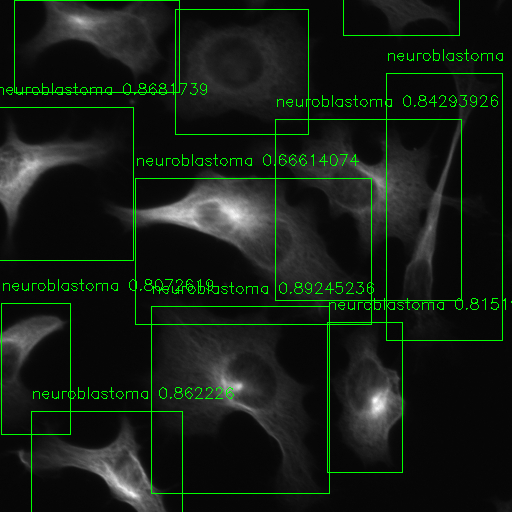
\includegraphics[width=\linewidth]{110084.png}
\end{subfigure}\vspace{2pt}
\begin{subfigure}[b]{0.9\linewidth}
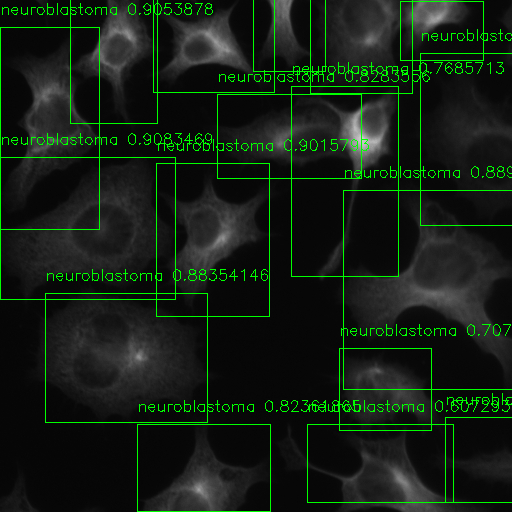
\includegraphics[width=\linewidth]{110085.png}
\end{subfigure}
\caption{\textbf{Neuroblastoma Detection}. Shown are some of the detected neuroblastoma cells using the Tiny YOLO network with the corresponding detection scores}
\label{fig:yolo_results}
\end{figure}
Detecting the neuroblastoma cells using the Tiny YOLO network proved to be an easy task. Figure \ref{fig:yolo_results} shows some of the boxed neuroblastoma cells in the test images.
Even with the highly irregular and dissimilar shape of the neuroblastoma cells, the trained detection network obtained an mAP of (value here).
\subsection{Neuroblastoma Semantic Segmentation}
While the Tiny YOLO network trained to detect neuroblastoma proved to be effective and efficient in its task, the segmentation it gives is a coarse one - a bounding box. For problems requiring pixel-level labelling of the cells, the output of YOLO is not enough. Here, we tried to combine the good cell localization of YOLO and the smoothing effect of conditional random fields to resolve pixelwise the cells and the background.


\subsection{Neuroblastoma Instance Segmentation}


\section{Conclusion}
The conclusion goes here.


% use section* for acknowledgment
\section*{Acknowledgment}


The authors would like to thank...


% Can use something like this to put references on a page
% by themselves when using endfloat and the captionsoff option.
\ifCLASSOPTIONcaptionsoff
  \newpage
\fi



% trigger a \newpage just before the given reference
% number - used to balance the columns on the last page
% adjust value as needed - may need to be readjusted if
% the document is modified later
%\IEEEtriggeratref{8}
% The "triggered" command can be changed if desired:
%\IEEEtriggercmd{\enlargethispage{-5in}}

% references section

% can use a bibliography generated by BibTeX as a .bbl file
% BibTeX documentation can be easily obtained at:
% http://mirror.ctan.org/biblio/bibtex/contrib/doc/
% The IEEEtran BibTeX style support page is at:
% http://www.michaelshell.org/tex/ieeetran/bibtex/
%\bibliographystyle{IEEEtran}
% argument is your BibTeX string definitions and bibliography database(s)
\bibliographystyle{IEEEtran}
\bibliography{ONBI_ROTATION_PROJECT1_DELASPENAS}
%
% <OR> manually copy in the resultant .bbl file
% set second argument of \begin to the number of references
% (used to reserve space for the reference number labels box)




% that's all folks
\end{document}


